\subsection{Decision Logic}

% [ERIC/KARTHIK - 1 pg]

% Decision logic, tabular spec and evolution, APT synth and proof \\

% might want to cite Alessandro's recent APT/ATJ/ATC papers?

A critical component of the RTA architecture is the Plan Selector, which selects flight
plans using formally verified decision logic. The Collins RTA RWC assessment
forwards the Plan Selector two plans, a plan generated by the LEC (``LEC plan'') and
the Backup Avoidance Flightplan (``BAF plan'') generated by the Backup Avoidance
Planner. After running the logic, the Plan Selector sends its decision to the
aircraft Plan Switch.

Given at most one LEC plan and one BAF plan, an assessment is made over five
general variables: plan validity (whether we've received the plan), plan
safety, whether the time of closest point of approach (tCPA) is greater than
179 seconds (the end of the planning horizon), comparison of the predicted miss
distance (pmd) of each plan, and whether 3 seconds has elapsed since the
receipt of the first plan (see Fig. \ref{fig:selection-logic}). If a plan is
not valid, we deem it unfit for publication.  If a plan is valid, and we've yet
to receive the other plan after 3 seconds, we go ahead and publish the plan we
received.  Otherwise, we've received two valid plans.  If exactly one of them
is safe, we publish it.  If neither plan is safe, we publish the one with the
larger predicted miss distance.  Otherwise, both plans are safe, so we consider
whether their times of closest approach are beyond the 179 second limit.  If
exactly one plan's tCPA is beyond the limit, we choose the other plan.  If
neither is beyond the limit, we chose the LEC plan.  Otherwise, both plans'
tCPA is beyond the 179 second limit.  In that case, we choose the plan with the
larger predicted miss distance.  See Fig. \ref{fig:selection-logic} for the
full decision table.

We formalized this decision table and applied our synthesis tools, based on the
ACL2 theorem prover\cite{acl2}, to synthesize high-assurance decision code
implementing the table logic.  This process used the $\verb+def-table+$
machinery described in \cite{dasc2020}.  In particular, proofs are
automatically performed on the table to ensure completeness (some case always
applies, and an output is always produced) and unambiguity (no more than one
case applies, so a unique output is always produced).

\begin{figure*}
	\centering
	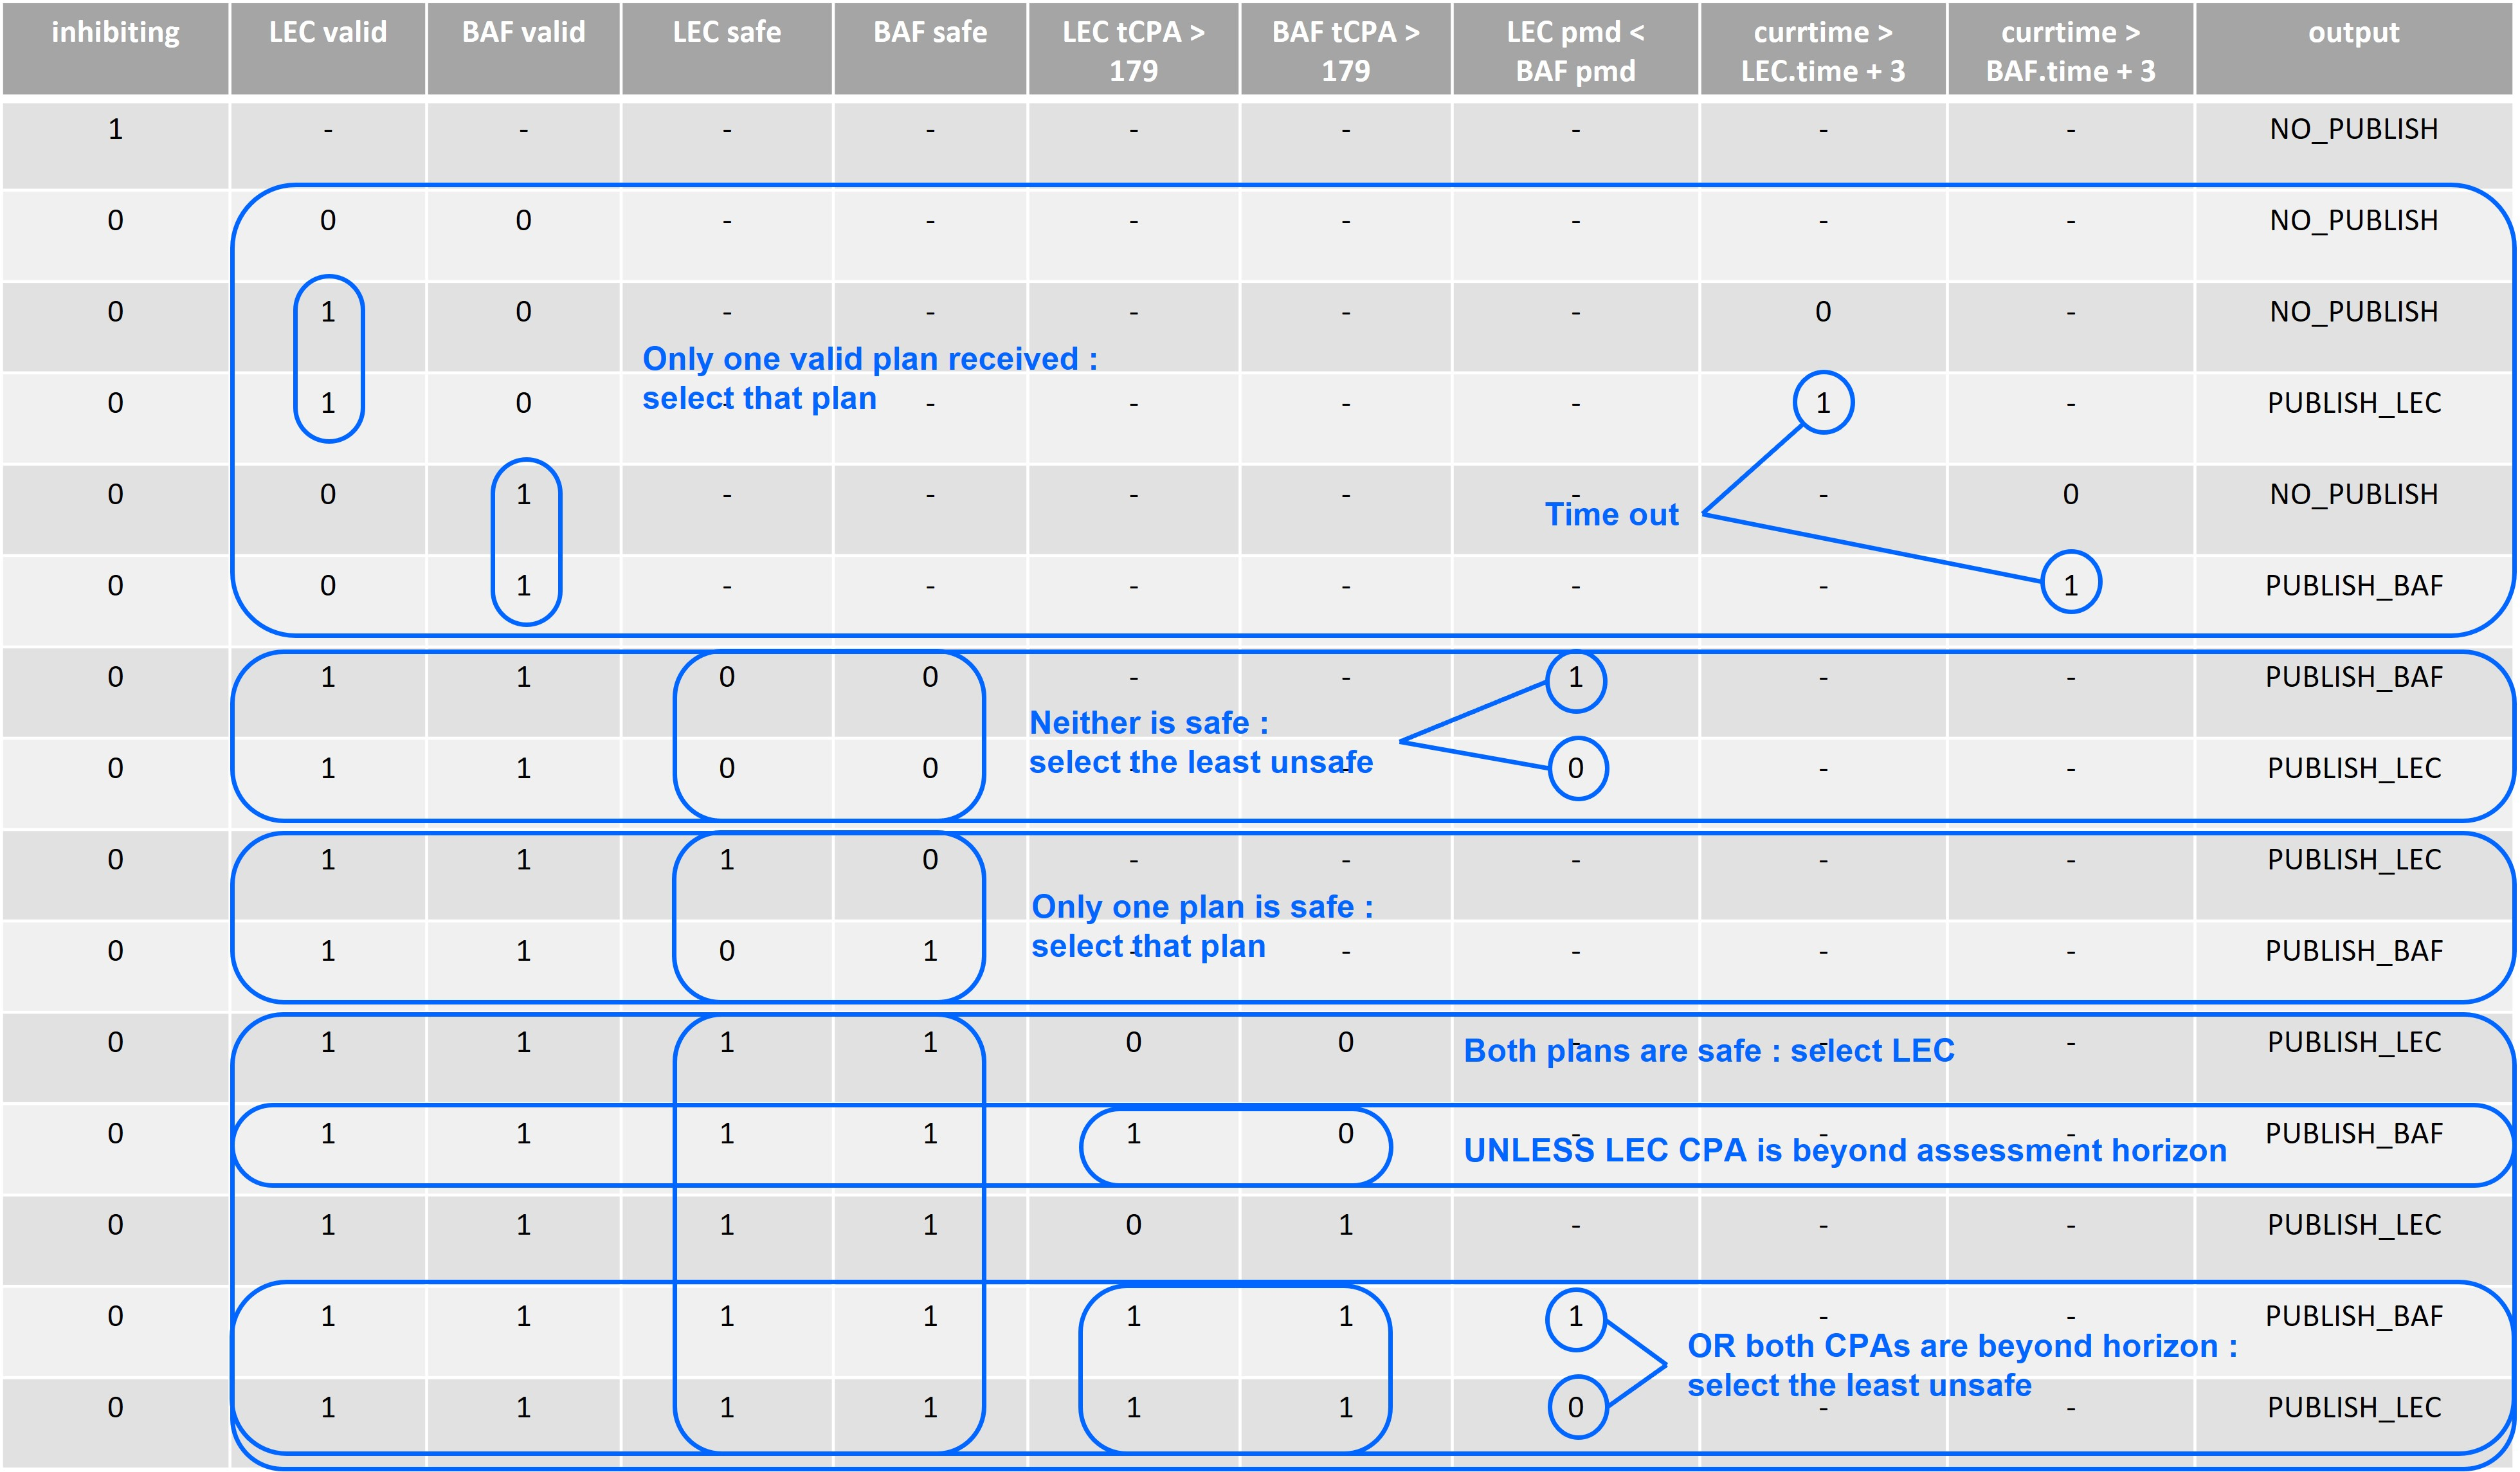
\includegraphics[width=\textwidth]{figures/selection-logic.jpg}
	\caption{Plan Selection logic specification (hyphens match either 0 or 1)}
	\label{fig:selection-logic}
\end{figure*}

Our software synthesis process starts with an executable specification that applies our generic table evaluation procedure \texttt{apply-table} to the specific table described above.  In this initial specification, the table is represented as a piece of data that is interpreted by \texttt{apply-table}.  Synthesis steps will specialize the table evaluation process, building in the specific table to create a cascade of conditional expressions.

We synthesize an executable Java program in two key steps:
\begin{enumerate}

\item Apply APT transformations to specialize and simplify the
  decision logic, creating an optimized, executable function: We use Kestrel's
  APT (Automated Program Transformations) \cite{apt} toolkit, built on ACL2,
  especially the \texttt{simplify} transformation, which applies simplifying
  rewrite rules from our library.
  %% Other synthesis steps
  %% include applications of our \texttt{letify}, and
  %% \texttt{lift-condition} transformations.
  %% \texttt{Letify} introduces \texttt{LET} constructs to bind variables and
  %% avoid re-computation, and \texttt{lift-condition} brings if-then-else
  %% expressions to the top level.
  Each of the APT transformation steps produces a proof showing the equivalence
  of its input and output.

\item Generate Java code using ATJ\cite{atj}: We use Kestrel's ATJ (ACL2-to-Java) Java
  code generator, built on ACL2, to generate Java code for integration with the
  Collins RTA.  Extending previous work (described in \cite{dasc2020}), ATJ now
  generates idiomatic and more performant Java code.

\end{enumerate}

For integration into the larger system, we created a hand-written wrapper for the generated Java decision code.  The wrapper receives and processes incoming plan messages from the Remain Well Clear Assessment, applies the generated decision code to the boolean plan variables, and publishes the decision to the Plan Switch.  Communication is done via ROS.

Our methodology for synthesizing the decision logic using program transformations allows for quick re-synthesis when the design changes.  One simply re-runs the synthesis tools using the new table-based specification as input.  This flexibility was demonstrated when simulations necessitated additional conditions and constraints on plan selection.  Specifically, the table was changed to consider whether each plan's tCPA exceeds the 179 second planning horizon. This simply amounted to changing the \texttt{def-table} encoding in ACL2, with all the correctness proofs, synthesis/optimization steps, and Java code generation following immediately.

Future improvements to this methodology may include:
\begin{itemize}
\item Outfitting ATJ with proofs: As remarked in \cite{dasc2020}, this might involve either formalizing the semantics of Java or using Kestrel's Axe toolkit to lift Java bytecode into logic.
\item Code generation for other languages (C, Python, Rust): Recent work at Kestrel was able to achieve the same synthesis presented above using the ATC C code generator\cite{atc} in place of ATJ, with the additional benefit of having proofs-of-correctness for the code generation.
\item Formal synthesis of RTA-logic interface: At the time of publication, the integration of the plan selection logic with the Collins RTA requires a handwritten wrapper, which could potentially also be synthesized with proofs.
\end{itemize}
